\subsection{Przegląd literatury}
\subsubsection{Wstęp}
Rozważania na temat inteligentnych systemów w kontekście niniejszej pracy należy zacząć od artykułu opublikowanego przez IBM w 2003 roku \cite{kephart2003}. Wskazuje on, iż ówczesne systemy informatyczne stają się coraz bardziej skomplikowane, co prowadzi do kryzysy zarządzania. Ręczna administracja przestaje być skalowalna, ponieważ systemy wymagają coraz większej liczby specjalistów do instalacji, konfiguracji oraz optymalizacji. IBM wskazuje, że jedyną opcją poradzenia sobie z tym problemem jest Autonomiczne Przetwarzanie (ang. \textit{Autonomic Computing}). Nawiązuje ono do autonomicznego układu nerwowego człowieka, który zarządza pracą naszego serca lub utrzymaniem temperatury ciała, zwalniając świadomą część mózgu z tych obowiązków. W kontekście systemów informatycznych człowiek zwolniony by był z konfiguracji, optymalizacji, naprawy oraz ochrony, gdyż powstałe system były by "Self-CHOP" (ang. \textit{Self-Configuration, Self-Optimization, Self-Healing, Self-Protection}). Jest to ważne pojęcie stanowiące podwaliny wielu dalszych badań. Architektura autonomicznych systemów przedstawiona jest na rysunku \ref{fig:24-ibm}.

\begin{figure}[!htbp]
    \centering 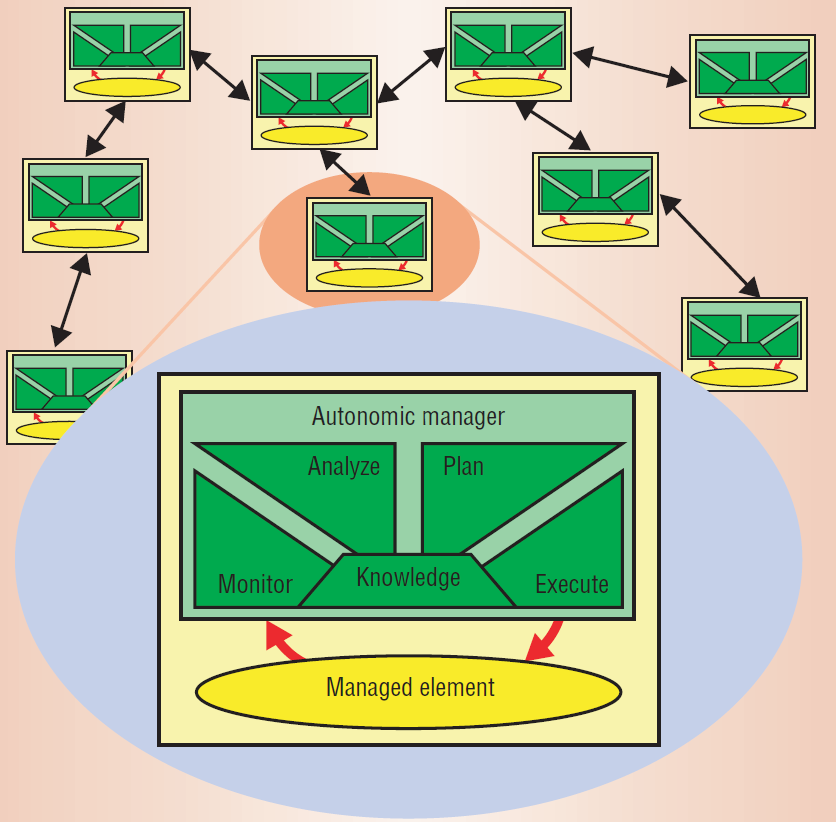
\includegraphics[width=1.0\linewidth]{24-ibm.png}
    \caption{Architektura autonomicznych systemów IBM}\label{fig:24-ibm}
\end{figure}

Podstawową jej jednostką jest element autonomiczny (ang. \textit{Autonomic Element}). Składa się on z zarządzanego komponentu (np. serwera, bazy danych, aplikacji czy urządzenia sieciowego) oraz autonomicznego menadżera (ang. \textit{Autonomic Manager}), który steruje jego działaniem. Menedżer autonomiczny działa w cyklu MAPE-K (Monitor, Analyze, Plan, Execute, Knowledge). Faza "Monitor" zbiera dane o zarządzanym obiekcie, które to są analizowane i oceniane pod względem potencjalnych problemów w fazie "Analyze". "Plan" odpowiada za rozpisanie działań naprawczych lub optymalizacyjnych, które są przekazywane do "Execute" w celu wdrożenia w systemie zarządzanym. "Knowledge" nie jest fazą a repozytorium wiedzy, do której każdy z elementów cyklu ma dostęp. Tu gromadzona jest \hyperlink{def:wiedza}{\textit{wiedza}}. Elementy autonomiczne mogą ze sobą współpracować i wymieniać się wiedzą. Inteligencja społeczna (ang. \textit{social intelligence}) całego rozproszonego systemu rośnie wraz z liczbą interakcji pomiędzy elementami, podobnie jak w kolonii mrówek. Gdy przyjdzie nowy element, to zdobywa wiedzę od reszty populacji. Widzimy tu lekką inspirację \cite{minsky1986}.

Następnie \cite{doyle2014} opisuje ewolucję architektury sieci telekomunikacyjnych w kierunku większej automatyzacji wymieniając czynniki umożliwiające (ang. \textit{enablers}) taki kierunek jako technologie: SDN (ang. \textit{Software Defined Networks}) oraz NFV (ang. \textit{Network Function Virtualization}).

Należy w tym momencie rozróżnić pojęcia Automatyzacji i Autonomiczności. Pierwsze odnosi się do predefiniowanego i zaprogramowanego procesu, podczas gdy drugie do aspektów związanych z samozarządzaniem. Zazwyczaj proces automatyczny nie jest w stanie zaadaptować się do zmian środowiska bez interwencji człowieka, co z kolei potrafi proces autonomiczny \cite{ngmn2022}. Czynnikiem technologicznym (ang. \text{enabler}) pozwalającym na przejście z automatyzacji na autonomiczność jest sztuczna inteligencja. \cite{benzaid2020} dokonuje przeglądu kierunków rozwoju badań na temat systemów ZSM. Czyli bezobsługowych systemów zarządzania siecią i usługami (ang. \textit{Zero-touch network and Service Management}), gdzie sztuczna inteligencja odgrywa kluczową rolę. Artykuł wymienia projekty organizacji standaryzujących w tym kierunku:
\begin{itemize}
    \item \textbf{ETSI GS ZSM} - specyfikuje referencyjną architekturę zarządzania siecią i usługami end-to-end. Framework ZSM jest postrzegany jako system zarządzania nowej generacji, który ma na celu pełną autonomiczność wszystkich procesów - od planowania, projektowania, dostarczania i wdrażanie, po udostępnianie, monitorowanie i optymalizację. Docelowo, w idealnym przypadku, powinien on działać w 100\% samodzielnie bez ingerencji człowieka. 
    \item \textbf{TM FORUM} - specyfikuje referencyjną architekturę CLADRA (Closed Loop Anomaly Detection and Resolution Automation) opartej o AI, która umożliwia dostawcom usług komunikacyjnych (CSP - ang. \textit{Communication Service Providers} na szybkie wykrywanie i rozwiązywanie problemów sieciowych.
    \item \textbf{ETSI GR ENI} - specyfikuje referencyjną architekturę kognitywnych systemów zarządzania siecią używając zamkniętych pętli sterowania oraz świadomych kontekstu polityk. O ile ETSI GS ZSM skupia się na technikach automatyzacji zarządzania oraz udostępniania usług end-to-end, to ENI koncentruje się na technikach AI, zarządzaniu poprzez polityki oraz zamkniętych pętlach sterowania.
\end{itemize}

Powyższe architektury zostaną dokładniej opisane w dalszej części pracy (zwłaszcza w części badawczej). Istotne na ten moment jest to, ze każda z tych architektur opiera swoje działanie o zamknięte pętle sterowania, co przewidział z resztą artykuł \cite{fallon2019}. Wskazuje on, iż badanie oraz stosowanie zamkniętych pętli sterowania jest dosyć starą dyscypliną sięgającą aż od ery pary \footnote{\url{https://en.wikipedia.org/wiki/Age_of_Steam}} (Rysunek \ref{fig:24-his}). Stosowane są one z powodzeniem w systemach morskich, lotniczych, motoryzacyjnych, przemysłowych ale też mikroprocesorach, systemach wbudowanych czy sterownikach urządzeń. Mimo że tego typu systemy są często złożone, cechują się determinizmem i dobrze określonymi granicami, co sprawia, że świetnie nadają się do zastosowania teorii sterowania\footnote{\url{https://en.wikipedia.org/wiki/Control_theory}}. Systemy telekomunikacyjne natomiast są słabo określonymi, stochastycznymi systemami, co sprawia, że zastosowanie teorii sterowania do ich zarządzania okazuje się wyjątkowo trudne. Stąd duże opóźnienie w ich adaptacji w branży telekomunikacyjnej. Od czasu pojawienia się propozycji Autonomicznego Zarządzania \cite{kephart2003} w 00s oraz enablerów w postaci SDN\&NFV w 10s zaczęły się pojawiać implementacje zamkniętych pętli sterowania w telekomunikacji. Niestety są one bardzo pragramtyczne i sztywne, skupione jedynie na dowożeniu danej funkcjonalności. Dodatkową problematyczność zagadnienia sprawia konieczność integracji systemów od wielu różnorodnych dostawców.

\begin{figure}[!htbp]
    \centering 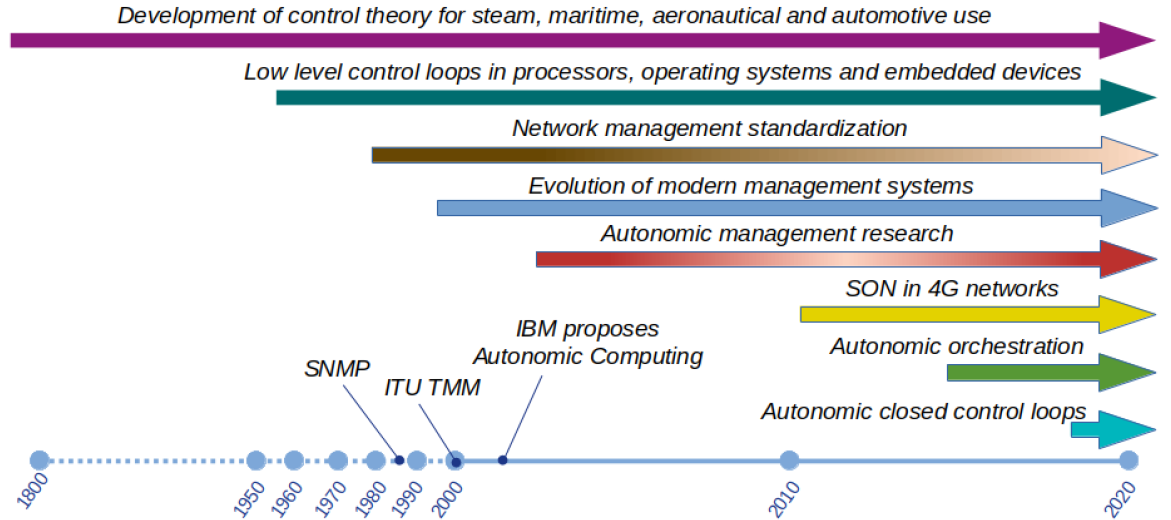
\includegraphics[width=1.0\linewidth]{24-his.png}
    \caption{Zestawienie lini czasu rozwoju systemów zarządzania siecią oraz pętli sterowania}\label{fig:24-his}
\end{figure}

\cite{fallon2019} wskazuje wyzwania jakim należy się przeciwstawić, aby umożliwić autonomiczność poprzez pętle sterowania w sieciach. Są to następujące kroki:
\begin{itemize}\hypertarget{list:1}{}
    \item Potrzebny jest model opisujący pętle sterowania w standardowy sposób. Pozwoli to uchronić się przed pragramtycznością i niesystematycznością.
    \item Potrzebny jest framework do wdrażania pętli sterowania umożliwiający ich zarządzanie oraz działanie (ang. \textit{runtime}) w jednym miejscu.
    \item Potrzebne są (najlepiej) graficzne narzędzia do projektowania i symulacji pętli sterowania, tak aby ich wdrażanie nie wymagało specjalistycznych umiejętności technicznych.
\end{itemize}

\subsubsection{ONAP/CLAMP}

Następnym punktem \cite{fallon2019} jest omówienie systemu zarządzania ONAP\footnote{\url{https://www.onap.org}} (Open Network Automation Platform) \cite{onap2018}. ONAP to open-source’owa platforma do orkiestracji, zarządzania i automatyzacji usług sieciowych, rozwijana przez Linux Foundation. ONAP składa się z \textbf{wielu modułów i API}, które umożliwiają pełne \textbf{zarządzanie cyklem życia usług sieciowych}, od ich projektowania, poprzez wdrażanie, aż po operacje eksploatacyjne. Jego kluczowe elementy to:
\begin{itemize}
    \item \textbf{Master Service Orchestrator (MSO)} – centralny komponent odpowiedzialny za orkiestrację.
    \item \textbf{SDN Controllers (APPC, SDNC, VFC)} – kontrolery zarządzające różnymi warstwami sieci.
    \item \textbf{A\&AI (Active and Available Inventory)} – komponent do zarządzania inwentaryzacją zasobów sieciowych.
    \item \textbf{DCAE (Data Collection, Analytics and Events)} – moduł do analizy danych i obsługi pętli sterowania.
    \item \textbf{CDS (Controller Design Studio)} – moduł do modelowania inteligentnych konfiguracji komponentów sieciowych
    \item \textbf{CLAMP (Control Loop Automation Management Platform)} – zarządza zamkniętymi pętlami sterowania.
\end{itemize}

Komponentem odpowiedzialnym za pętle sterowania w ONAP jak i zarówno kandydatem na przeciwstawiennictwo wyzwaniom postawionym powyżej jest CLAMP\footnote{\url{https://docs.onap.org/projects/onap-policy-parent/en/istanbul/clamp/clamp/clamp-architecture.html}}. Ma on jednak swoje ograniczenia:
\begin{itemize}
    \item Wymaga stosowania architektury pętli zgodnej z MAPE-K, co ogranicza możliwość wdrożenia nietypowych pętli sterowania.
    \item Wymaga ścisłej integracji z innymi modułami ONAP takimi jak DCAE, CDS, czy silniki polityk, co ogranicza możliwości tworzenia pętli niezależnych od ekosystemu ONAP.
    \item Jest zoptymalizowany do prostych pętli sterowania. Brak natywnego wsparcia dla bardziej złożonych architektur jak pętle hierarchiczne, rozproszone lub współzależne.
    \item Brak wsparcia AI/ML w swoich komponentów.
    \item Ścisłe połączenie z wybranymi silnikami polityk takimi jak XACML \footnote{\url{https://docs.onap.org/projects/onap-policy-parent/en/istanbul/xacml/xacml.html}}, Drools\footnote{\url{https://docs.onap.org/projects/onap-policy-parent/en/istanbul/drools/drools.html}} czy APEX \footnote{\url{https://docs.onap.org/projects/onap-policy-parent/en/istanbul/apex/apex.html}} 
    \item Ścisła specjalizacja w orkiestracji sieci SDN\&NFV. Ciężko jest rozwijać pętle, które nie są związane z tym zagadnieniem.
\end{itemize}




\subsubsection{Architektura referencyjna ETSI ZSM}\hypertarget{sec:zsm}{}
Nadrzędnym celem projektowym ZSM jest umożliwienie nie wymagającego udziału człowieka (ang. \textit{zero touch}) zarządzania siecią i usługami w środowisku wielu dostawców (ang. \textit{multi-vendor environment}) \cite{etsizsm2018}. Architektura przyjmuje pewien zestaw pryncypiów (zasad):
\begin{enumerate}\hypertarget{list:2}{}
    \item Modularność  
    \item Rozszerzalność  
    \item Skalowalność  
    \item Sterowane modelem, otwarte interfejsy  
    \item \textbf{Automatyzacja zarządzania w pętli zamkniętej}  
    \item Obsługa funkcji zarządzania bezstanowego  
    \item Odporność  
    \item Rozdzielenie obszarów zarządzania  
    \item Kompozycyjność usług  
    \item Interfejsy oparte na intencjach  
    \item Abstrakcja funkcjonalna  
    \item Prostota  
    \item Zaprojektowane do automatyzacji  
\end{enumerate}

Framework ZSM podąża za trendem w branży polegającym na odejściu od monolitycznych ściśle powiązanych systemów na rzecz bardziej elastycznych zestawów usług zarządzania (ang. \textit{management services}). Referencyjna architektura ZSM określa zestaw elementów składowych (ang. \textit{building blocks}), które wspólnie umożliwiają konstruowanie bardziej złożonych usług i funkcji zarządzania. Konstrukcja ta odbywa się zgodnie ze wzorcami kompozycji i współdziałania (ang. \textit{composition and interoperation patterns}). 

Logicznie, framework ZSM składa się z rozproszonych serwisów zarządzania (ang. \textit{management services} i serwisów danych (ang. \textit{data services}), które zorganizowane są w domeny zarządzania (ang. \textit{management domains}) oraz zintegrowane poprzez powłokę integracyjną (ang. \textit{integration fabric}). Powłoka integracyjna również jest uzywana do komunikacji serwisów zarządzania z systemami zewnętrznymi.

Architektura referencyjna zapewnia środki do budowania i komponowania luźno powiązanych funkcji zarządzania (ang. \textit{management functions}), które oferują serwisy zarządzania i wspólnie zapewniają kompleksowe zarządzanie danej domeny w sposób "zero-touch". Aby oferować swoje serwisy, funkcje udostępniają możliwość ich wywoływania i komunikacji z nimi za pomocą end-point'ów. 

\begin{figure}[!htbp]
    \centering 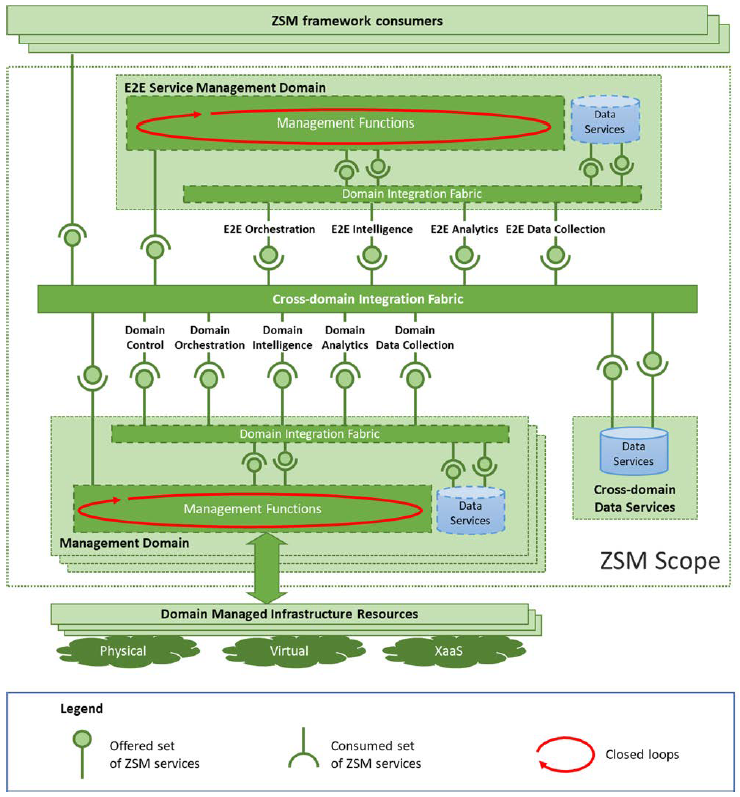
\includegraphics[width=1.0\linewidth]{24-zsm-arch.png}
    \caption{Architektura referencyjna ZSM}\label{fig:24-zsm-arch}
\end{figure}

Na rysunku \ref{fig:24-zsm-arch} przedstawiono architekturę referencyjną. Poniżej krótkie omówienie jej elementów:
\begin{itemize}
    \item Serwis zarządzania (ang. Management Service) - niewidoczna na rysunku, najmniejsza jednostka usługowa architektury, odpowiedzialna za niepodzielny aspekt składowy zarządzania
    \item Serwis danych (ang. Data Service) - jednostka odpowiedzialna za gromadzenie danych, informacji oraz wiedzy
    \item Funkcja zarządzania (ang. Management Function) - połączenie wielu serwisów zarządzania, odpowiedzialna za dany aspekt składowy zamkniętej pętli zarządzania
    \item Domena Zarządzania (ang. Management Domain) - odpowiedzialna za konkretną funkcjonalność zarządzania (np. analityka, orkiestracja, bezpieczeństwo)
    \item Domena Zarządzania end-to-end (ang. E2E Management Domain) - odpowiedzialna za zarządzanie usługami wymagającymi wielu funkcjonalności
    \item Powłoka integracji (ang. Integration Fabric) - odpowiedzialna za komunikacje pomiędzy między wszystkimi komponentami
\end{itemize}

Pętle zarządzania komponowane są z funkcji zarządzania w sposób pokazany na rysunku \ref{fig:24-zsm-loop}. Jako model przyjęto  strukturę pętli OODA \cite{boyd1995} z wprowadzeniem komponentu wiedzy znanego z pętli MAPE-K \cite{kephart2003}. 

\begin{figure}[!htbp]
    \centering 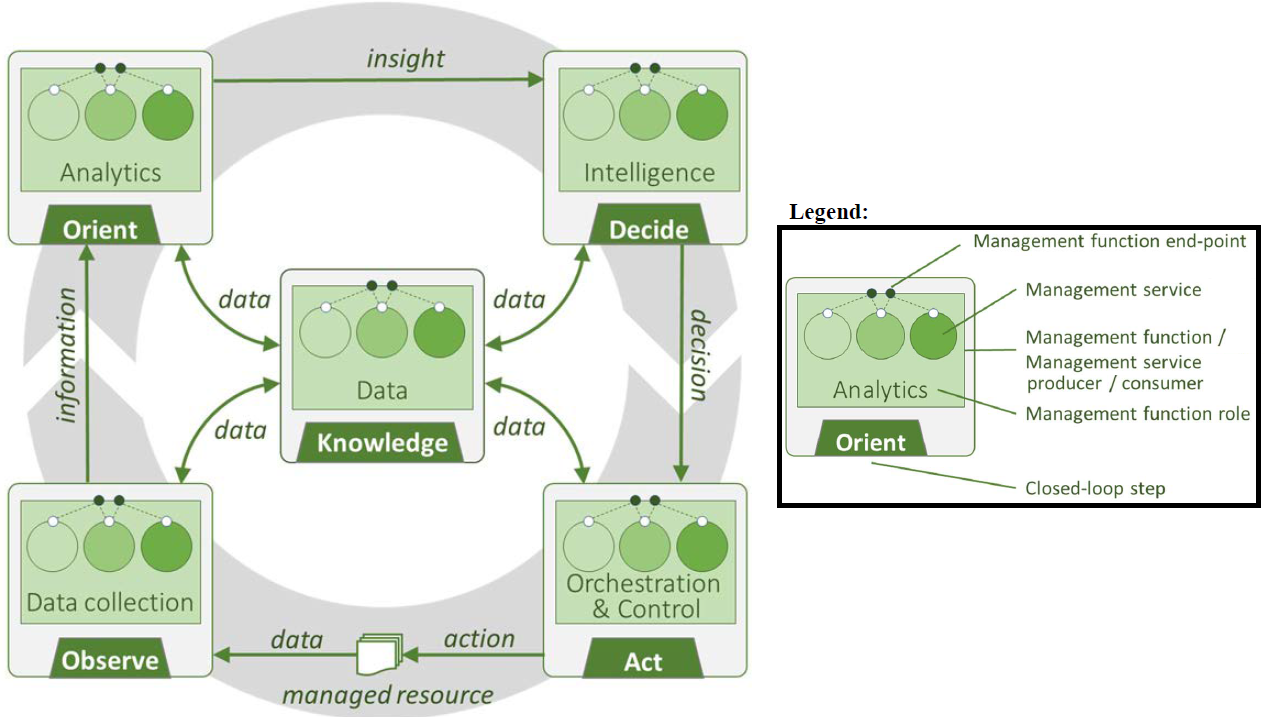
\includegraphics[width=1.0\linewidth]{24-zsm-loop.png}
    \caption{Mapowanie pomiędzy elementami składowymi architektury ZSM a zamkniętą pętlą sterowania}\label{fig:24-zsm-loop}
\end{figure}


Architektura ZSM również specyfikuje cykl życia zamkniętej pętli sterowania oraz koordynacje między pętlami. Cykl życia pętli podzielony jest na dwie fazy: "Design-Time" oraz "Run-Time" a ich poszczególne kroki obserwujemy na rysunku \ref{fig:24-zsm-lifecycle}. Jeśli chodzi o koordynacje między pętlami to zdefiniowano dwa przypadki: pętle hierarchiczne oraz pętle peer-to-peer. Pętle mogą komunikować się w obrębie jednej domeny zarządzania jak i również między domenami. 

\begin{figure}[!htbp]
    \centering 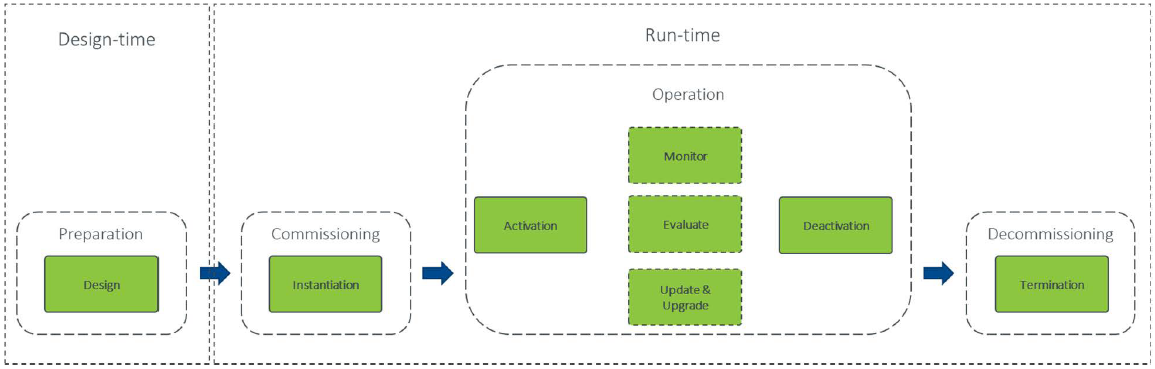
\includegraphics[width=1.0\linewidth]{24-zsm-lifecycle.png}
    \caption{Fazy cyklu życia oraz aktywności zamkniętej pętli sterowania}\label{fig:24-zsm-lifecycle}
\end{figure}




\subsubsection{Architektura referencyjna CLADRA (TM Forum)}\hypertarget{sec:cladra}{}

TM Forum specyfikuje architekturę referencyjną, która w oparciu o zamknięte pętle sterowania pomaga szybko wykrywać oraz rozwiązywać problemy występujące w sieciach. Podobnie jak architektura ETSI ZSM jest oparta o Open Digital Architecture (ODA) \cite{tmforum2018}. Nie jest to jednak specyfikacja techniczna tak jak w przypadku ETSI. 

W \cite{tmforum2021} przedstawiono architekturę logiczną (Rysunek )

\begin{figure}[!htbp]
    \centering 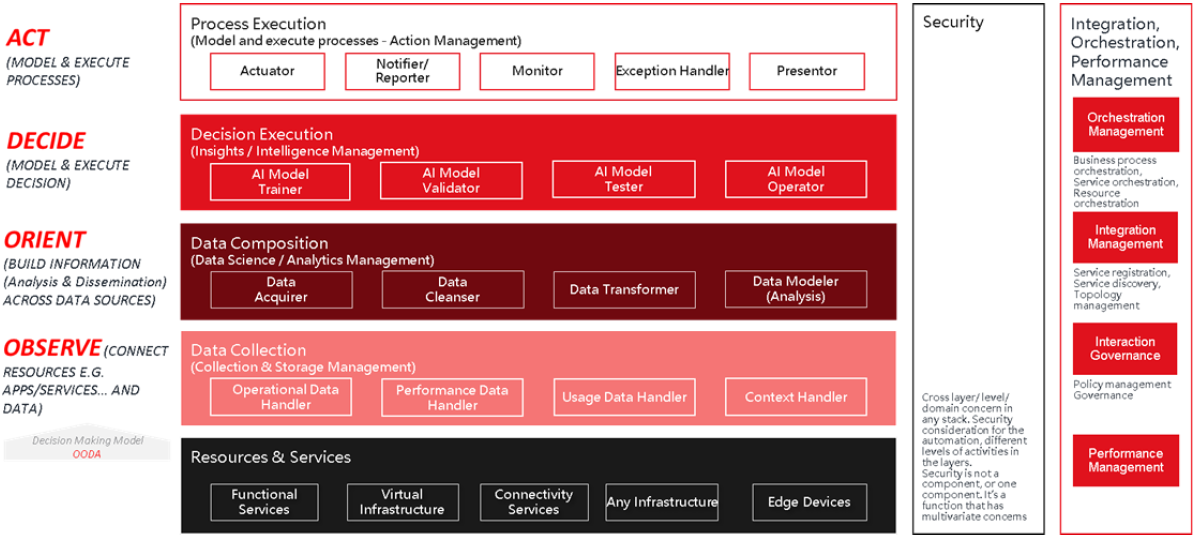
\includegraphics[width=1.0\linewidth]{24-tmforum-arch.png}
    \caption{Architektura logiczna CLADRA}\label{fig:24-tmforum-arch}
\end{figure}

Opiera się ona na pętli OODA. Krok "Observe" jest odpowiedzialny za zbieranie danych z sieci, na podstawie których w drodze analizy budowana jest informacja w fazie "Orient". W kroku "Decide" podejmowane i modelowane są decyzje, które przekładają się na konkretne workflow do wykonania. Krok "Act" orkiestruje wykonaniem workflow na zarządzanych zasobach. Warto zwrócić tu uwagę na aspekt, iż workflow akcji rekoncylacyjnych do wykonania jest dopiero wnioskowane podczas iteracji pętli (w kontraście do workflow zdefiniowanego przed runtime danej iteracji). Jest to architektura na innym poziomie abstrakcji niż architektura ZSM. Konkretne jej implementacje przedstawione w \cite{tmforum2022} różnią się bardzo od siebie i tak jak wskazano w \cite{fallon2019} są bardzo sztywne i skierowane na dany use-case. Natomiast podobnie jak architektura ETSI ZSM przewidywane jest uruchamianie na jednej platformie wielu różnych instancji pętli jednocześnie. Celem tych pętli jest autonomiczne zarządzanie realizowane za pomocą komunikacji z zewnętrznymi względem tej platformy zasobami. 

\cite{tmforum2022ai} prezentuje koncepcję Menedżera Zamkniętych Pętli (ang. \textit{Closed Loop Manager}), czyli komponentu architektury odpowiedzialnego za zarządzanie pętlami sterowania. Podobna kwestia poruszana jest również przez \cite{ngmn2022}. Taki menadżer w kontekście pętli sterowania jest odpowiedzialny za:
\begin{itemize}
    \item Zarządzanie ich cyklem życia 
    \item Konfiguracji ich celów zarządzania
    \item Monitorowanie ich stanu
\end{itemize}

Pełna tabela funkcjonalności proponowanych dla Menadżera Zamkniętych Pętli przez TM Forum znajduje się w \hyperlink{appendix:11}{Załączniku 11}.

\subsubsection{Achitektura referencyjna ETSI ENI}

ENI rozwija specyfikacje w kierunku Kognitywnego Systemu Zarządzania, który będzie samodzielnie regulował działanie sieci poprzez wykorzystanie technik sztucznej inteligencji, takich jak \hyperlink{def:uczenie-maszynowe}{uczenie maszynowe (ang. \textit{machine learning})} oraz \hyperlink{def:wnioskowanie}{wnioskowanie (ang. \textit{reasoning})}. 

Z poprzedniej sekcji wiemy, że aby \hyperlink{def:wnioskowanie}{\textit{wnioskować}} potrzebna jest \hyperlink{def:wiedza}{\textit{wiedza}}. Skąd taki system pozyskiwałby wiedzę? Otóż, dzieje się to poprzez proces \hyperlink{def:uczenie-maszynowe}{\textit{Uczenia Maszynowego}}. Pierwsza faza czyli tzw. "trening", odbywa się jeszcze przed wdrożeniem systemu. Ale system również może uczyć się "z doświadczenia" (ang. \textit{experience}), kiedy już jest w pełni operacyjny. Stąd mówimy o empirycznej inteligencji sieciowej (ang. \textit{experiential networked intelligence}). 

Architekturę \cite{etsieni2023} ENI obrazuje Rysunek \ref{fig:24-eni-arch}. Fioletowe komponenty są zewnętrzne dla systemu ENI: górny stanowi jednostki zlecające mu zarządzanie, zaś dolny zarządzany obiekt (w tym przypadku zarządzana infrastruktura). Miedzy nimi występują pętle zarządzania end-to-end, co jest podobnym konceptem jak w przypadku ETSI ZSM. Oba komponenty zewnętrzne, z racji, że sieci telekomunikacyjne są środowiskiem z wieloma dostawcami (ang. \textit{multi-vendor environment}), muszą przejść normalizację formatu danych (lub/i interfejsów) na jeden ogólny format rozumiany przez ENI System (tzw. ENI Format). Odpowiedzialne za to są dwa czerwone komponenty. Prawdziwym punktem kluczowym architektury jest komponent zielony. To w nim dokonywane są operacje zarządzania oparte na sztucznej inteligencji. Całość cyklu zamknięta jest pętlą sterowania. 

Podczas gdy ZSM specyfikuje framework do orkiestracji i egzekwowania działań w sieci, to ENI może działać jako warstwa kognitywna dla ZSM. ZSM realizuje zamknięte pętle sterowania, reagując na konkretne działa w czasie rzeczywistym. ENI analizuje długoterminowe trendy i dynamicznie dostosowuje polityki zarządzania w celu np. zapobiegania anomalii sieciowych. Kognitywność ENI również opiera się na zamkniętych pętlach sterowania i co ważne z punktu widzenia niniejszej pracy \cite{etsieni2024} dokonuje przeglądu różnych architektur zamkniętych pętli sterowania, które mogą zostać użyte w ENI System. Stanowi on świetne źródło wiedzy o charakterystykach zamkniętych pętli sterowania. Jego analiza znajduje się w \hyperlink{sec:25}{następnej podsekcji}.



\begin{figure}[!h]
    \centering 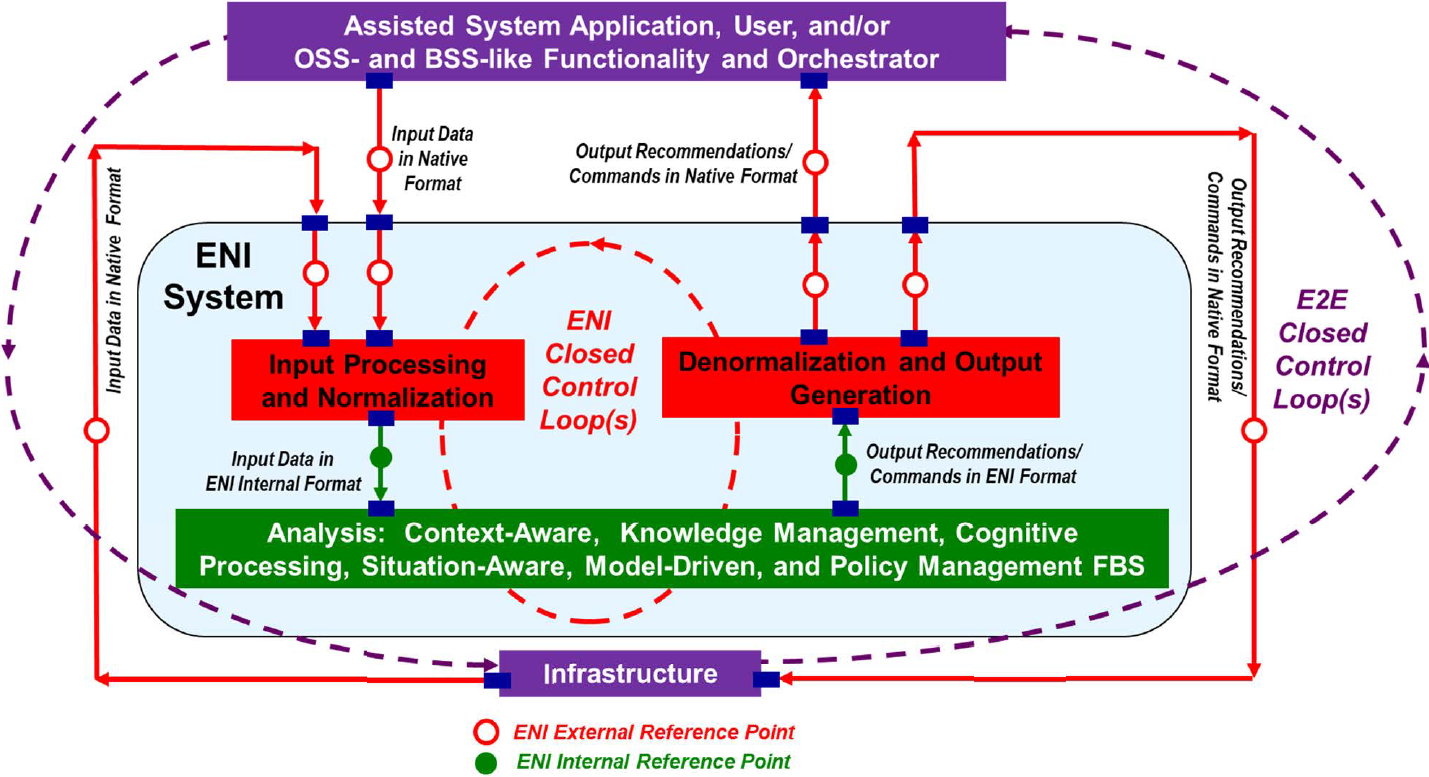
\includegraphics[width=1\linewidth]{24-eni-arch.png}
    \caption{Wysokopoziomowa architektura funkcjonalna ENI}\label{fig:24-eni-arch}
\end{figure}


\subsubsection{Podsumowanie}

Niniejsza praca znajduję lukę, którą chce zapełnić w postaci platformy służącej do modelowania oraz uruchamiania zamkniętych pętli sterowania. Luka ta umotywowana jest \hyperlink{list:1}{wyzwaniami zdefiniowanymi przez \cite{fallon2019}}, brakami w ONAP/CLAMP oraz zidentyfikowanie potrzeby takiej platformy w architekturach referencyjnych definiowanych przez ETSI GS ZSM oraz CLADRA.

Odnosząc się do architektury z \cite{kephart2003} proponowana w niniejszej pracy platforma polega na wyniesieniu autonomicznych menadżerów do jednego wspólnego miejsca (Rysunek \ref{fig:24-lupus}).

\begin{figure}[!htbp]
    \centering 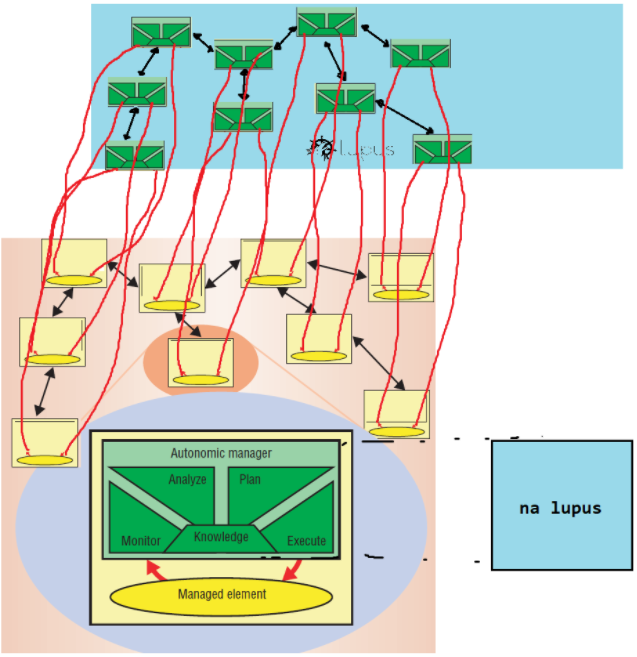
\includegraphics[width=1.0\linewidth]{24-lupus.png}
    \caption{Koncepcja wyniesienia autonomicznych menadżerów na wspólną platformę (//TODO)}\label{fig:24-lupus}
\end{figure}